\problemname{Dance Pad}
A dance pad consists of four arrows pointing up, right, down and left.
When playing a dance game you are given a sequence of arrows to step on to the beat of the music.
Sometimes two arrows can be shown for the same beat, so you have to make a jump to step on them.
You can always remain on an arrow with a foot even if you don't need to press it for a beat.

\begin{figure}[ht!]
    \centering
    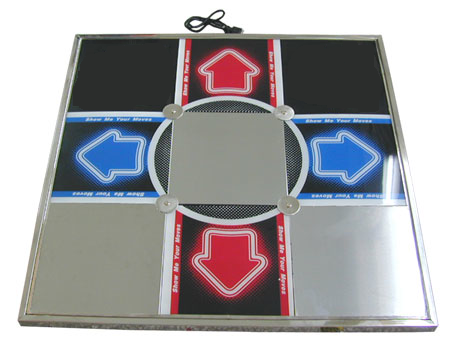
\includegraphics[width=0.4\textwidth]{dansmatta.png}
\caption{A dance pad.}
\label{fig:sample1}
\end{figure}

Johan jumps around on his dance pad almost every day, but finds it hard to keep up with moving his feet sometimes.
Therefore he wants some help with playing a song optimally.
That means moving his feet to new arrows as few times as possible.

At the start of the game, his left foot is on the left arrow, and his right foot on the right arrow.

Given a song and which \emph{one or two} arrows have to be pressed at each beat, compute the minimum number of times Johan must move a foot to another arrow.
Moving both his feet in a jump still counts as two movements.


\section*{Input}
The first line contains the integer $N$ ($1 \le N \le 10\,000$), the number of beats in the song.

This is followed by $N$ lines, one line for each beat.
Each beat consists of a string with \emph{one or two} letters of \texttt{U}, \texttt{H}, \texttt{N} or \texttt{V} meaning ``up'', ``right'', ``down'', ``left'', respectively.
These are the arrows that must be pressed during the beat.

\section*{Output}
Output the an integer -- the least number of moves Johan must make.

\section*{Scoring}
Your solution will be tested on a set of test case groups.
To get the points for a group, you need to pass all the test cases in the group.

\noindent
\begin{tabular}{| l | l | p{10cm} |}
\hline
Group & Points & Constraints \\ \hline
  $1$    & $20$        & $N \le 10$ and Johan only needs to press one arrow per beat. \\ \hline 
  $2$    & $30$        & Johan only needs to press one arrow per beat. \\ \hline
  $3$    & $50$        & No further constraints. \\ \hline 
\end{tabular}

\section*{Explanation of sample 1}
Johan starts with his feet on the left and right arrows (as always).
A possible optimal solution is the following.
For the first beat, he moves the right foot to the up arrow.
Then he moves the right foot again to the down arrow.
For the next two moves he doesn't move his feet, since he already have a foot on the left arrow, and finally he moves an arbitrary foot to the right arrow.
This requires $3$ moves.
